\documentclass[../DS06.tex]{subfiles}
\graphicspath{{./figures/}}

% \subimport{/home/nora/Documents/Enseignement/Prepa/bpep/exercices/DS/lentille_magnetique/}{sujet.tex}

\begin{document}
\prblm[91]{Lentillage magnétique\ifcorrige{~\footnotesize\textit{(D'après Banque
			PT 2017 et capes 2008)}}}

\enonce{
	La microscopie optique classique est limitée par la diffraction. Pour
	améliorer la résolution, on remplace les photons par des électrons de charge
	$q = -e$ et de masse $m$.
}

\QR[3]{%
	Définir la diffraction. Donner, en argumentant, un ordre de grandeur de la
	résolution d'un microscope optique fonctionnant dans le visible.
}{%
	La diffraction est un phénomène ondulatoire se produisant lors de
	l'interaction d'une onde de longueur d'onde $\lambda$ avec un objet de
	dimension \pt{1} comparable à $\lambda$. La diffraction d'une onde engendre un
	étirement spatial \pt{1} de l'onde.

	La résolution d'un microscope optique est donc de l'ordre de la longueur
	d'onde du visible, soit \pt{1} $\SIrange{400}{800}{nm}$.
}

\begin{center}
	\vspace{15pt}
	\fbox{\Large Les trois parties sont indépendantes.}
\end{center}

\partie{Aspect énergétique}
\enonce{
	\noindent
	\begin{isd}
		Les électrons sont accélérés dans un canon à électrons
		(figure~\ref{fig:canon}) constitué de deux armatures planes et parallèles,
		distantes de $d = \SI{1}{cm}$ et séparées par du vide quasi-parfait.
		\smallbreak
		On applique entre les armatures une tension positive $U = V_1-V_2$. On
		suppose que le champ électrique $\Ef$ entre les armatures est uniforme.
		\tcblower
		\begin{center}
			\input{./figures/canon.pdf_tex}
			\captionof{figure}{Schéma du canon à électrons.}
			\label{fig:canon}
		\end{center}
	\end{isd}
}

\QR[5]{%
	Représenter le champ électrique $\Ef$ entre les armatures. Sur quelle
	armature les électrons doivent-ils être émis sachant que leur vitesse initiale
	est nulle~? Exprimer la force électrique exercée sur l'électron en fonction de
	$E_0 = \norm{\Ef}$, $e$ et $\uz$.
}{%
	\smallbreak
	\vspace{-15pt}
	\noindent
	\begin{isd}
		Le champ électrique est orienté selon les potentiels décroissants \pt{1}, donc
		$\boxed{\Ef \stm[-1]{=} -E_0\uz}$.
		\smallbreak
		La force électrique s'exerçant sur l'électron s'écrit $\vv{F_e} \stm[-1]{=}
			-e\Ef = eE_0\uz$. Cette force est orientée selon $+\uz$, donc les électrons
		doivent être \xul{émis depuis l'armature 2.} \pt{1}
		\tcblower
		\begin{center}
			\input{./figures/canoncorr.pdf_tex}
			\captionof{figure}{Schéma complété \protect\pt{1}}
		\end{center}
	\end{isd}
	\vspace{-15pt}
}

\QR[3]{%
	Déterminer l'expression de l'énergie potentielle électrique $\Ec_p(z)$ de
	l'électron situé à la distance $z$ de l'armature 2 en fonction de $z$, puis
	écrire la relation entre $\Ec_p(z)$ et le potentiel $V(z)$. Montrer alors que
	$E_0 = \frac{U}{d}$ et donner l'expression de $\Ef$.
}{%
	\smallbreak
	\vspace{-15pt}
	\noindent
	\begin{isd}[interior hidden]
	\vspace{-15pt}
		\begin{gather*}
			\de{W}(\Ff_e) \stm{=} \Ff_e \cdot \dd{\OM} \stm[-1]{=} -\dd{\Ec_p}
			\\\Lra
			eE_0 \dd{z} = - \dd{\Ec_p}
			\\\Lra
			-\dd(-eE_0z) = -\dd{\Ec_p}
			\\
			\beforetext{Ainsi}
			\boxed{\Ec_p \stm[-1]{=} -eE_0z + \cte}
		\end{gather*}
		\tcblower
	\vspace{-15pt}
		\begin{gather*}
			\beforetext{Or,}
			\Ec_p(z) \stm[-1]{=} -eV(z)
			\\\Ra
			\Ec_p(d)-\Ec_p(0) = -e(V(d)-V(0)) = -eU
			\\
			\beforetext{Or}
			\Ec_p(d)-\Ec_p(0) = -eE_0d~~\pt{1}
			\\
			\beforetext{Donc}
			E_0 = U/d
			\Ra
			\boxed{\Ef \stm{=} -\dfrac{U}{d}\uz}
		\end{gather*}
	\end{isd}
	\vspace{-15pt}
}

\enonce{
	On donne les valeurs numériques approchées~:
	\[
		\cfrac{e}{m}\approx \SI{2e11}{SI}\qet \cfrac{h}{m}\approx \SI{7e-4}{SI}
	\]
	où $h$ est la constante de Planck intervenant à la question~\ref{Q:planck}.
}

\QR[7]{%
	Exprimer la vitesse $v$ atteinte par les électrons lorsqu'ils arrivent sur
	l'armature opposée, en fonction de $U$, $e$ et $m$. Calculer $v$ sachant que
	$U = \SI{1e5}{\volt}$. Commenter l'ordre de grandeur obtenu.
}{%
	L'électron, assimilable à un point matériel $M$ de masse $m$, est étudié dans
	le référentiel du laboratoire supposé galiléen \pt{1}. Il n'est soumis qu'à la
	force électrique (on néglige le poids \pt{1}) qui est une force conservative
	\pt{1}. Donc $\Ec_m = \cte$ \pt{1}. Ainsi entre $z = 0$ et $z = d$~:
	\begin{gather*}
		\Ec_m(0) = -eV(0)
		\quad \stm{\text{et}} \quad
		\Ec_m(d) = -eV(d)+\cfrac{1}{2}mv^2
		\\\Ra
		\boxed{v \stm{=} \sqrt{\cfrac{2eU}{m}}}
		\qar
		U = V(d)-V(0)
		\\\AN
		\xul{v \stm[-1]{=} \SI{2e8}{m.s^{-1}}}
	\end{gather*}
	Donc la particule est relativiste.
}

\enonce{%
	On utilisera pour la question suivante la définition de la quantité de
	mouvement dans l'hypothèse d'une particule non-relativiste. On peut montrer
	qu'en considérant la particule comme étant relativiste, on aboutit à une
	longueur d'onde du même ordre de grandeur.
}

\QR[2]{\label{Q:planck}
	On donne la relation de \textsc{de Broglie} définissant la longueur d'onde
	d'une particule quantique~: $p = h/\lambda$, avec $p$ la quantité de mouvement
	de la particule. Calculer la longueur d'onde $\lambda$ associée aux électrons
	ainsi accélérés.
}{%
	Pour une particule non-relativiste, $p = mv$ \pt{1}, donc $\xul{\lambda =
			\SI{3,5e-12}{\meter}}$ \pt{1}.
}

\partie{Déflecteur magnétique}
\enonce{
	Le rôle d'un déflecteur magnétique est simplement de dévier le faisceau
	d'électrons.

	On suppose qu'un électron de vitesse $\vfo$ arrive dans une zone où règne
	un champ magnétique uniforme $\Bf$ perpendiculaire au vecteur vitesse. Il
	n'y a plus de champ électrique.
}

\QR[4]{%
	Établir le système puis justifier le fait que le mouvement de l'électron est
	uniforme.
}{%
	\vspace{-15pt}
	\begin{itemize}
		\bitem{Système}~: {électron}, assimilé à un point matériel de masse $m$ et
		de charge $q$, référentiel du laboratoire supposé galiléen. \pt{1}
		\bitem{BDF}~:
		\vspace{-15pt}
		\[
			\begin{array}{ll}
				\textbf{Poids}                     &
				\text{négligeable \pt{1} \textbf{devant }}\Ff \\
				\textbf{Force de \textsc{Lorentz}} &
				\Ff \stm[-1]{=} -e(\Ef + \vf\wedge\Bf)
			\end{array}
		\]
	\end{itemize}
	À l'intérieur du déflecteur, seule la force magnétique $\Ff_m =
		e\vf\wedge\Bf$ existe. Ainsi, d'après le TPC,
	\[
		\dv{\Ec_c}{t} \stm[-1]{=}
		-e\underbracket[1pt]
		{\underbracket[1pt]
			{\vf\wedge\Bf}_{\perp\vf}\cdot\vf}_{=0} \stm[-1]{=} 0
		\qsoit
		mv\dv{v}{t} = 0
		\qMath{d'où}
		\boxed{\dv{v}{t} \stm[-1]{=} 0}
	\]
	Ainsi la trajectoire est uniforme.
}

\QR[4]{%
	On admet que la trajectoire est circulaire. On travaillera dans le repère $(C,
		\ur,\ut,\uz)$ avec $C$ le centre du cercle. Donner le répérage et exprimer
	$\af$ en fonction de $v_0$ puis tracer cette trajectoire, en faisant
	clairement apparaitre les vecteurs $\vfo$, $\Bf$ et $\Ff(0)$.
	\smallbreak
	Placer le centre $C$ de la trajectoire circulaire, ainsi que la base polaire
	$(\ur,\ut)$ de centre $C$. L'axe de référence pour l'angle $\th$ sera pris
	parallèle à $\vfo$ et passant par $C$.
}{%
	\smallbreak
	\vspace{-15pt}
	\noindent
	\begin{isd}
		\begin{center}
			\input{./figures/circulaire.pdf_tex}
			\captionof{figure}{Schéma \protect\pt{2}}
		\end{center}
		\tcblower
		\begin{gather*}
			\OM = R \ur
			\\\Ra
			\vf = R\tp\ut
			\\\Ra
			\af \stm[-1]{=}
			\underbracket{R\tpp}_{\mathclap{=0~\text{car uniforme}}}\ut - R\tp^{2}\ur
			\\\Lra
			\boxed{\af \stm[-1]{=} -\frac{v_0{}^{2}}{R}\ur}
		\end{gather*}
	\end{isd}
}

\QR[3]{%
	Déterminer l'expression du rayon $R$ du cercle décrit en fonction de $m$,
	$v_0$, $e$ et $B$.
}{%
	\vspace{-25pt}
	\begin{gather*}
		\beforetext{PFD~:}
		m\af \stm[-1]{=} \Ff_m
		\\\Lra
		-\frac{mv_0{}^{2}}{R}\ur = -q v_0\ut \wedge B\uz \stm[-1]{=} -ev_0B\ur
		\\\Lra
		\boxed{R \stm{=} \frac{mv_0}{eB}}
	\end{gather*}
}

\partie{Lentille magnétique}
\enonce{
	Le contrôle de la focalisation du faisceau électronique dans le microscope
	électronique est possible en utilisant des lentilles magnétiques. On
	s'intéresse ici à une lentille magnétique, modélisée par une bobine de $N$
	tours confondus, circulaires de rayon $a$, de centre $O$, d'axe $Oz$ et
	parcourue par un courant permanent $I$. Cette bobine est obtenue par
	l'enroulement d'un fil électrique.
	\smallbreak
	En considérant les symétries et les invariances du bobinage, on peut justifier
	que le champ magnétique est indépendant de $\th$ et ne possède pas de
	composante orthoradiale (selon $\ut$). On peut alors écrire~:
	\[
		\Bf(M) = B_r(r,z)\er+B_z(r,z)\ez
	\]
	En pratique, le faisceau électronique passe dans le domaine $r\ll a$. Dans ce
	cas, on peut se contenter d'une expression approchée du champ $\Bf$ au
	voisinage de l'axe $Oz$~:
	\[
		\boxed{\Bf(M)\approx -\cfrac{r}{2}\,\dv{B_z(0,z)}{z}\er+B_z(0,z)\ez}
	\]
	\begin{isd}[righthand ratio=.4]
		avec $B_z(0,z) = \frac{B_0}{\left( 1+{z^2}/{a^2} \right)^{3/2}}$ le
		champ magnétique sur l'axe $Oz$ et $B_0 = \frac{\mu_0NI}{2a}$ le champ
		magnétique en $O$.
		\smallbreak
		Un point $M$ de l'espace sera repéré par ses coordonnées cylindriques $(r,
			\th, z)$ d'axe $Oz$ et de centre~$O$. On place en un point $P$ de l'axe $Oz$,
		en amont de la lentille magnétique, une source ponctuelle d'électrons. On
		considère un électron émis depuis le point $P$ avec une vitesse $\vfo$.
		\smallbreak
		On ajoute les hypothèses simplificatrices suivantes à l'étude~:
		\tcblower
		\begin{center}
			\input{./figures/coordonnees.pdf_tex}
			\captionof{figure}{Schématisatioon.}
		\end{center}
	\end{isd}
	\begin{itemize}
		\item L'électron est supposé non relativiste.
		\item L'électron ne subit que la force magnétique due à la lentille.
		\item Le vecteur vitesse initial $\vfo$ en $P$ est dans le plan méridien
		      $\th = 0$ et forme un angle $\alpha$ avec l'axe~$Oz$.
		\item L'angle $\alpha$ est faible ($\alpha\ll 1$) et la trajectoire
		      ultérieure de l'électron reste dans le domaine~$r\ll a$.
	\end{itemize}
}

\QR[3]{%
	À quelle approximation d'optique une de ces hypothèses fait-elle penser~? On
	définira cette approximation et on précisera les conséquences.
}{%
	La dernière hypothèse fait penser aux conditions de \textsc{Gauss} \pt{1}
	consistant à ne considérer que des rayons paraxiaux (proches de l'axe optique
	et faiblement inclinés par rapport à celui-ci). \pt{1}

	Dans ces conditions, il y a stigmatisme et aplanétisme approchés. \pt{1}
}

\QR[5]{%
	Déterminer l'ordre de grandeur de la valeur de champ magnétique à partir de
	laquelle on peut ne pas tenir compte du poids de l'électron dans l'étude de
	son mouvement. On supposera que l'ordre de grandeur de la vitesse de
	l'électron est \SI{1e8}{m.s^{-1}}. Conclure.
}{%
	L'ordre de grandeur de la force magnétique est $F_m = evB$ \pt{1}. Le poids
	s'exprime $P = mg$ \pt{1}. On veut que $P/F_m\ll 1$~:
	\begin{gather*}
		\cfrac{mg}{evB}\stm{\ll} 1
		\quad \Leftrightarrow \quad
		\boxed{B \stm{\gg} \cfrac{mg}{ev}}
		\\\AN
		\xul{B \stm[-1]{\gg} \SI{5e-19}{T}}
	\end{gather*}
	Il faut donc que $B$ soit supérieur à \SI{5e-19}{\tesla}, ce qui est une
	valeur extrêmement faible. Donc il est raisonnable de négliger le poids.
	\pt{1}
}

\QR[4]{%
Exprimer l'accélération de $M$ en coordonnées cylindriques, puis montrer que
sa composante orthoradiale (selon $\ut$) peut être mise sous la forme
$\DS\dfrac{1}{r}\dv{t}\pac{r^2\tp}$.
}{%
On donne le repérage en coordonnées cylindriques~:
\[
\OM \stm[-1]{=} r \er + z \ez
\quad \Ra \quad
\vf \stm[-1]{=} \rp \er+r\tp\et+\zp \ez
\quad \Ra \quad
\af \stm[-1]{=} (\rpp -r(\tp)^2)\er+(r\tpp+2\rp  \tp)\et+\zpp \ez
\]
On remarque que l'accélération orthoradiale peut s'écrire sous la forme~:
\[
\cfrac{1}{r}\dv{t}\left[r^2\dv{\th}{t}\right] \stm{=}
\cfrac{1}{r}(2r\rp \tp+r^2\tpp) = 2\rp \tp+r\tpp
\]
}

\QR[6]{%
	En utilisant le résultat précédant, en déduire les trois équations
	différentielles du mouvement, que l'on notera (1), (2) et (3) et qui
	correspondent respectivement à la projection du principe fondamental de la
	dynamique sur $\er$, $\et$ et $\ez$. Expliciter toutes les dérivées
	temporelles avec des $\dv{t}$.
}{%
	On exprime la force de Lorentz dans la base cylindrique~:
	\[
		\vv{F_m} = -e\vf\wedge\Bf = -e
		\begin{pmatrix}
			\rp  \\
			r\tp \\
			\zp
		\end{pmatrix}
		\wedge
		\begin{pmatrix}
			-\cfrac{r}{2}\,\dv{B_z(0,z)}{z} \\
			0                               \\
			B_z(0,z)
		\end{pmatrix} = -e
		\begin{pmatrix}
			r\tp B_z(0,z)                                    \pt{1} \\
			-\cfrac{r}{2}\,\dv{B_z(0,z)}{z}\zp -\rp B_z(0,z) \pt{1} \\
			-r\tp\left(-\cfrac{r}{2}\,\dv{B_z(0,z)}{z}\right) \pt{1}
		\end{pmatrix}
	\]
	En projetant le PFD dans la base cylindrique, on obtient les équations~:
	\begin{align}
		\label{eq:1}\dv[2]{r}{t}-r\left( \dv{\th}{t} \right)^2
		 & \stm{=}
		-\cfrac{e}{m}\,r\,\dv{\th}{t}B_z(0,z)
		\\
		\dv{}{t}\left[r^2\dv{\th}{t}\right]
		 & \stm{=}
		\label{eq:2}
		\cfrac{e}{m}\,r\left[
			\dv{r}{t}B_z(0,z) + \cfrac{r}{2}\,\dv{z}{t}\,\dv{B_z(0,z)}{z}
			\right]
		\\
		\label{eq:3}
		\dv[2]{z}{t}
		 & \stm{=}
		-\cfrac{e}{2m}\,r^2\,\dv{\th}{t}\,\dv{B_z(0,z)}{z}
	\end{align}
}

\QR[3]{%
	Montrer que l'équation~(2) peut s'écrire
	\[
		\dv{t}\pac{r^{2}\dv{\th}{t}} = \frac{e}{2m} \dv{t}\pac{r^{2}B_z(0,z)}
	\]
	En déduire la relation $\DS\dv{\th}{t} = \cfrac{e}{2m}B_z(0,z)$.
}{%
	Le second membre de l'équation~\eqref{eq:2} peut s'écrire~:
	\begin{align*}
		\cfrac{e}{2m}\,\dv{}{t}\left[ r^2B_z(0,z) \right]
		                    & =
		\cfrac{e}{2m}\left[ 2r\rp B_z(0,z)+r^2\zp  \dv{B_z(0,z)}{z} \right]
		\\
		                    & \stm{=}
		\cfrac{e}{m}\,r\left[\dv{r}{t}B_z(0,z) +
			\cfrac{r}{2}\,\dv{z}{t}\,\dv{B_z(0,z)}{z} \right]
		\\
		\beforetext{Par intégration de l'équation~\eqref{eq:2},}
		r^2\dv{\th}{t}
		                    & \stm{=}
		\cfrac{e}{2m}\,r^2B_z(0,z) +\cte
		\\\beforetext{Or}
		r(t=0) = 0
		                    & \Ra
		\cte = 0 \pt{1}
		\\\Lra
		\Aboxed{\dv{\th}{t} & = \cfrac{e}{2m}B_z(0,z)}
	\end{align*}
}

\QR[6]{%
	L'équation~(3) présente un second membre en $r^2$ négligeable dans le cadre de
	cette étude (car d'ordre 2 en $r/a$). Que vaut alors $\dv{z}{t}$~? On rappelle
	que l'angle $\alpha$ est faible.
	\smallbreak
	En déduire, en partant de l'équation~(1), que l'évolution radiale $r(z)$ de
	l'électron vérifie l'équation différentielle
	\begin{equation}
		\dv[2]{r}{z}+\cfrac{e^2}{4m^2v_0^2}\,\,rB_z^2(0,z) = 0\label{eq:rz}
	\end{equation}
}{%
	Par intégration de l'équation~\eqref{eq:3}, $\boxed{\dv{z}{t} = \cte =
			v_0\cos(\alpha)\stm{\approx} v_0}$. Par l'équation~\eqref{eq:1}, en remplaçant
	$\tp$ par son expression~:
	\begin{gather*}
		\rpp -r\cfrac{e^2}{4m^2}\,B^2_z(0,z) \stm{=}
		-\cfrac{e}{m} r\times \cfrac{e}{2m}B_z(0,z)\times B_z(0,z)
		\quad\Leftrightarrow \quad
		\rpp +r\cfrac{e^2}{4m^2}B^2_z(0,z) \stm{=} 0
		\\
		\beforetext{Or}
		\dv{r}{t} \stm[-1]{=} \dv{r}{z}\cdot\dv{z}{t}\approx v_0\dv{r}{z}
		\\\Ra
		\dv[2]{r}{t}\approx v_0\dv[2]{r}{z}\dv{z}{t}
		\stm{\approx} v_0^2\dv[2]{r}{z}
		\\
		\beforetext{Ainsi}
		\boxed{\dv[2]{r}{z}+\cfrac{e^2}{4m^2v_0^2}\,\,rB_z^2(0,z) \stm{=} 0}
	\end{gather*}
}

\QR[4]{%
	On propose sur les figures~\ref{fig:tracer1} et~\ref{fig:tracer2} deux
	familles de tracés de fonctions $r(z)$ partant d'un point d'annulation avec un
	angle de départ $\alpha$ variable. Quelle figure représente effectivement un
	champ de solutions possible de l'équation~\eqref{eq:rz} (on justifiera la
	réponse)~? Le système étudié joue-t-il bien son rôle attendu de lentille~?
	\smallbreak
	\begin{isd}
		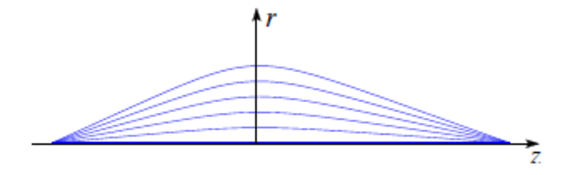
\includegraphics[width=.8\linewidth]{lentille1}
		\captionof{figure}{Proposition 1 de $r(z)$.}
		\label{fig:tracer1}
		\tcblower
		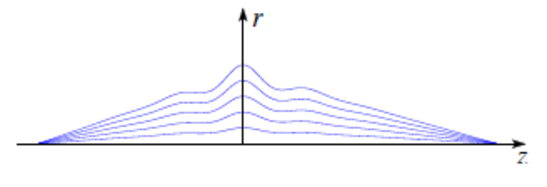
\includegraphics[width=.8\linewidth]{lentille2}
		\captionof{figure}{Proposition 2 de $r(z)$.}
		\label{fig:tracer2}
	\end{isd}
}{%
	D'après l'équation~\eqref{eq:rz}, $\boxed{\dv[2]{r}{z}<0}$ \pt{1}, donc la
	courbe $r(z)$ est forcément \xul{concave} \pt{1}. Cette constatation est en
	accord avec la figure de gauche. \pt{1}
	\smallbreak
	On constate que les courbes $r(z)$ s'annulent en un point de l'axe $Oz$, avec
	$z>0$. Ce point $P'$ est le conjugué du point $P$ \pt{1}. Donc le système joue
	bien le rôle d'une lentille.
}

\enonce{
	On ajoute à présent l'hypothèse de lentille mince, c'est-à-dire que le champ
	magnétique du bobinage n'intervient que sur une zone faible d'épaisseur
	comprise entre deux plans $\Pi$ et $\Pi'$, de positions $-z_0$ et $z_0$ avec
	$z_0\ll OP$ (figure~\ref{fig:schemalentille}).
	\smallbreak
	\noindent
	\begin{isd}
		Dans ces conditions, on peut montrer que la distance focale est
		approximativement donnée par
		\[
			f' = \cfrac{32m^2v_0^2}{3\pi ae^2B_0^2}
		\]
		Dans ce cadre, on peut toujours écrire que
		\begin{gather*}
			\dv{\th}{t} = \cfrac{e}{2m}B_z(0,z)
		\end{gather*}
		et l'équation différentielle sur le mouvement radial $r(z)$ est utilisable
		sous la forme approchée
		\[
			\dv[2]{r}{z}\approx -\cfrac{e^2}{4m^2v_0^2}\,r_0B_z^2(0,z)
		\]
		où $r_0$ est une valeur approchée de $r(z)$ (à l'ordre zéro en $r/a$) entre
		les plans $\Pi$ et $\Pi'$.
		\tcblower
		\begin{center}
			\input{./figures/schemalentille.pdf_tex}
			\captionof{figure}{Schéma de la lentille mince.}
			\label{fig:schemalentille}
		\end{center}
	\end{isd}
}
\QR[2]{%
	Pourquoi la trajectoire d'un électron seul est forcément rectiligne en dehors
	de la zone de champ magnétique~?
}{%
	En dehors de la zone de champ magnétique, l'électron n'est soumis qu'au poids
	qui est négligeable devant tout éventuel résidu de champ magnétique, donc à
	aucune force \pt{1}. Donc d'après le principe d'inertie, il est animé d'un
	mouvement de translation rectiligne uniforme. \pt{1}
}

\QR[6]{%
	Exprimer l'angle d'incidence $\alpha$ de l'électron en fonction de $r_0$ et de
	la distance algébrique $\obarr{OP}$. Attention au sens de comptage positif des
	angles. L'exprimer alors comme une valeur de $\DS \dv{r}{z}$ en un certain
	point.
	\smallbreak
	On note $P'$ le point de focalisation du rayon électronique, issu de la
	lentille, sur l'axe $Oz$ et on pose $\alpha'$ l'angle d'émergence de la zone
	magnétique. Préciser sur une figure l'angle $\alpha'$ et son orientation, et
	exprimer de même $\alpha'$ en fonction de $r_0$ et de $\obarr{OP'}$ puis en
	fonction de $\DS \dv{r}{z}$.
}{%
	\[
		\tan(\alpha) \stm{=}
		-\cfrac{r_0}{\obarr{OP}} \stm{\approx}
		\alpha \stm{=} \dv{r}{z}\/(-z_0)
		\qqet
		\alpha' \stm{>} 0 \Ra
		\tan(\alpha') \stm{=}
		-\frac{r_0}{\obarr{OP'}} \stm{=}
		\dv{r}{z}\/(z_0)
	\]
}

\QR[7]{%
	Montrer alors que le
	système vérifie une loi de conjugaison de Descartes de lentille mince de
	centre $O$ et de focale $f'$ telle que
	\[
		\cfrac{1}{\obarr{OP'}}-\cfrac{1}{\obarr{OP}} = \cfrac{1}{f'}
		\qqav
		\cfrac{1}{f'} = \cfrac{e^2}{4m^2v_0^2}\int_{-z_0}^{+z_0}B_z^2(0,z)\dd z
	\]
}{%
	\vspace{-15pt}
	\begin{align*}
		\frac{1}{\obarr{OP'}} - \frac{1}{\obarr{OP}}                  & \stm{=}
		\frac{-1}{r_0}\left( \alpha' - \alpha\right)
		\\
		\beforetext{Or}
		\alpha' - \alpha                                              & =
		\dv{r}{z}\/(z_0)-\dv{r}{z}\/(-z_0) \stm{=}
		\int_{-z_0}^{z_0}\dv[2]{r}{z}\dd z
		\\
		\beforetext{De plus}
		\int_{-z_0}^{z_0}\dv[2]{r}{z}\dd z                            & \stm{=}
		-\cfrac{e^2r_0}{4m^2v_0^2}\int_{-z_0}^{+z_0}B_z^2(0,z)\dd z
		\\
		\beforetext{Ainsi}
		-r_0\left(\cfrac{1}{\obarr{OP'}}-\cfrac{1}{\obarr{OP}}\right) & =
		-\cfrac{e^2r_0}{4m^2v_0^2}\int_{-z_0}^{+z_0}B_z^2(0,z)\dd{z}
		\\\Lra
		\Aboxed{
		\cfrac{1}{\obarr{OP'}}-\cfrac{1}{\obarr{OP}}                  & \stm{=}
			\cfrac{e^2}{4m^2v_0^2}\int_{-z_0}^{+z_0}B_z^2(0,z)\dd{z}
		}
		\\
		\beforetext{On pose alors la distance focale}
		\cfrac{1}{f'}                                                 & = \cfrac{e^2}{4m^2v_0^2}\int_{-z_0}^{+z_0}B_z^2(0,z)\dd z
	\end{align*}
}

\QR[4]{%
	Montrer que, pendant le passage de l'électron dans la zone de champ
	magnétique, l'électron ne reste pas dans un même plan et qu'il y a un
	angle de rotation $\Delta \th$ autour de l'axe $Oz$ de la trajectoire de
	l'électron qui vaut
	\[
		\Delta \th = \cfrac{e}{2mv_0}\int_{-z_0}^{z_0}B_z(0,z)\dd z
	\]
}{%
	\[
		\dv{\th}{t} \stm{=} \dv{\th}{z}\,\dv{z}{t}\approx \dv{\th}{z}v_0
		\qdc
		\dv{\th}{z} \stm{=} \cfrac{1}{v_0}\dv{\th}{t} = \cfrac{e}{2mv_0}B_z(0,z)
	\]
	On intègre par rapport à $z$~:
	\[
		\Delta \th \stm{=}
		\int_{-z_0}^{z_0}\dv{\th}{z}\,\dd z \stm{=}
		\cfrac{e}{2mv_0}\int_{-z_0}^{z_0}B_z(0,z)\dd z
	\]
}

\enonce{
	Dans le cas de la spire, les intégrales pouvant être étendues de $-\infty$ à  $+\infty$, un calcul non demandé donne
	\[
		\Delta \th = \cfrac{aeB_0}{mv_0}
	\]
}

\QR[2]{%
	Quel est le signe de $f'$~? Conclure.
}{%
	$f'>0$ \pt{1}, donc la lentille est convergente \pt{1}.
}

\QR[2]{%
	Sur quels paramètres peut-on jouer pour réduire $f'$ à tension accélératrice
	$U$ fixée~?
}{%
	Pour diminuer $f'$, il faut augmenter $aB_0^2 = \cfrac{N^2I^2}{a}$. On peut
	augmenter l'intensité $I$ \pt{1}, ou diminuer le rayon $a$ \pt{1} des spires.
}

\QR[2]{%
	On donne $B_0 = \SI{1.0}{T}$, $a = \SI{1.0}{mm}$ et on choisit la tension
	accélératrice $U$ de sorte que ${v_0 = \SI{2.0e8}{m.s^{-1}}}$. Calculer $f'$
	et $\Delta \th$.
}{%
	\vspace{-15pt}
	\begin{gather*}
		\xul{f' \stm[-1]{=} \SI{3,4}{mm}}
		\qet
		\xul{\Delta \th \stm[-1]{=} \SI{1}{rad} = \ang{57}}
	\end{gather*}
}

\QR[4]{%
	Les aberrations interviennent aussi avec une lentille magnétique. Il existe
	notamment l'aberration dite «~de charge d'espace~» qui n'existe pas en optique
	classique. Quelle en est selon vous l'origine~? Pourquoi la réduction de cette
	aberration passe par l'utilisation de faisceaux électroniques peu denses~?
}{%
	Les électrons sont des particules chargées \pt{1} pouvant interagir entre eux
	par l'interaction électromagnétique. Ce n'est pas le cas des photons \pt{1}
	qui sont des particules non chargées.

	La répulsion \pt{1} entre les électrons rend la focalisation du faisceau
	électronique plus difficile. Cet effet est d'autant plus important \pt{1} que
	le faisceau électronique est dense.
}

\end{document}
